\documentclass[12px]{article}
\usepackage[cjk]{kotex}
\usepackage[top=2cm, bottom=4.5cm, left=2.5cm, right=2.5cm]{geometry}
\usepackage{amsmath, amssymb}
\usepackage{enumerate}
\usepackage{graphicx}
% \usepackage{tikz}
% \addtolength{\oddsidemargin}{-.875in}
% \addtolength{\evensidemargin}{-.875in}
% \addtolength{\textwidth}{1.75in}
% \addtolength{\topmargin}{-.875in}
% \addtolength{\textheight}{1.75in}

\title{응용통계학 4장 연습문제 풀이}
\author{20181653 이강희}
\date{}

\begin{document}
\maketitle

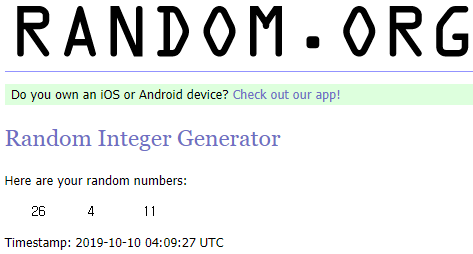
\includegraphics[scale=0.7]{random}

\section*{4번}
0점부터 시작해서 5점씩 20문제를 맞출 수 있다.\\
확률변수 X가 가질 수 있는 값은 0, 5, 10, ..., 100 이 있다.

\section*{11번}
\begin{enumerate}[(1)]
    \setlength\abovedisplayskip{0pt}
    \item
    \begin{minipage}[t]{\linewidth}
    \vspace{-\baselineskip}
    \begin{flalign*}
        P(X<4) &= \int_2^4 f(x) dx&\\
        &= \int_2^4 \frac{2(1+x)}{27} dx\\
        &= \left[\frac{2}{27}x + \frac{1}{27}x^2 \right]_2^4\\
        &= \frac{8}{27} + \frac{16}{27} - \left(\frac{4}{27} + \frac{4}{27}\right) = \frac{16}{27}
    \end{flalign*}
    \end{minipage}
    \item
    \begin{minipage}[t]{\linewidth}
    \vspace{-\baselineskip}
    \begin{flalign*}
        P(3<X<4) &= \int_3^4 f(x) dx&\\
        &= \int_3^4 \frac{2(1+x)}{27} dx\\
        &= \left[\frac{2}{27}x + \frac{1}{27}x^2 \right]_3^4\\
        &= \frac{8}{27} + \frac{16}{27} - (\frac{6}{27} + \frac{9}{27}) = \frac{1}{3}
    \end{flalign*}
    \end{minipage}
\end{enumerate}
\section*{26번}
\begin{flalign*}
    E(X) &= \int_{0}^{\infty} x \frac{1}{4}e^{\frac{-x}{4}} dx&\\
    &= \left[-xe^{-\frac{x}{4}} - 4e^{-\frac{x}{4}} \right]_{0}^{\infty}\\
    &=4\\
\end{flalign*}
\begin{flalign*}
    E(X^2) &= \int_{0}^{\infty} x^2 \frac{1}{4}e^{-\frac{x}{4}} dx&\\
    &= \left[-e^{-\frac{x}{4}}(x^2+8x+32) \right]_{0}^{\infty}\\
    &=32\\
\end{flalign*}
\begin{flalign*}
    \sigma_x^2 &= E(X^2) - E(X)^2&\\
    &= 32 - 4^2 = 16
\end{flalign*}
Y의 평균은 \(E(Y) = E(3X-2) = 3E(X)-2 = 10\)\\
Y의 분산은 \(\sigma_y^2 = \sigma_{3x-2}^{2} = 3^2\sigma_x^2\) = 144

\end{document}